\documentclass[a4paper,12pt]{article}
\usepackage{graphicx}
\usepackage{float}
\usepackage{amsmath}
\usepackage{graphicx}

\graphicspath{ {./media/} }
\hyphenpenalty 1000

\begin{document}

\title{
	A  Multi-Modal Visual and Text Based Approach to Multi-Page Document Classification.\\
	\bigbreak
	\Large MSc Data Science Project
}

\author{Justin Boylan-Toomey \\ Birkbeck, University of London\\ \\Project Supervisor \\Felix Reidl }
\date{October, 10, 2020}
\maketitle

\newpage

\begin{center}
\noindent\textbf{Academic Declaration}\\
\noindent I have read and understood the sections of plagiarism in the College
Policy on assessment offences and confirm that the work is my own, with
the work of others clearly acknowledged. I give my permission to submit
my report to the plagiarism testing database that the College is using
and test it using plagiarism detection software, search engines or
meta-searching software.

\end{center}

\newpage

\tableofcontents

\newpage

\section{Introduction}
\subsection{Document Classification}

The automatic classification of documents remains an important and only partially solved information management problem within the upstream oil and gas industry. Companies in this sector have typically amassed vast repositories of unstructured data measuring in the range of tens to thousands of terabytes. These repositories consist of data relating to their past hydrocarbon exploration and production activities, partnerships, acquisitions or more recently the digitisation of their physical legacy data archives. An estimated 80\% of all data within the upstream oil and gas industry is stored within these large unstructured document repositories (Bilnston, 2017).\\

Retrieving relevant documents from these large unstructured data repositories is a major challenge for the industry, with some reports suggesting that geoscientists and engineers spend over 50\% of their time searching for data (Mohammadpoor, 2018). Locating specific data types such as porosity and permeability logs, well trajectories and composite wireline logs can be challenging. Many of the document types found in such repositories are vital to informing exploration and risk management decisions, as well as to ensuring regulatory compliance. If crucial data is omitted from exploration models due to difficulties in its retrieval, this can lead to costly dry exploration wells or jeopardise the safety of a company’s operations.\\

Automated document classification algorithms aid information retrieval from these repositories by automatically identifying documents that fall within a defined set of useful document types. These classifiers act in a similar manner to static search queries, which when combined with key word search, allow results to be refined to only include the data types a user is seeking to retrieve. The predicted classifications when used more broadly can also assist in providing data management oversight of the data within these repositories. \\

Recently, supervised machine learning has been widely used to create these algorithmic classifiers. With the machine learning algorithm learning a document classification prediction function from a pre-labelled corpus of representative documents. Historically these classifiers can learn document classifications at a granular level based on a documents text content or at a higher level based on image representations of their pages. However the use of only a single modality such as text or visual feature representations presents challenges to effectively classifying oil and gas documents, some documents may lack text content or have a high visual similarity to those in another class. Recently multi-modal classifiers have been proposed that make use of both text and image features to classify documents and have been shown to be promising at overcoming similar challenges in document classification within other domains such as banking (Rusinol, 2014).  \\

This work explores the use of multi-modal deep neural network classifiers for the classification of multi-page oil and gas documents, combing both the text and visual modalities to in theory provide a more robust classification algorithm. Uni-modal and multi-modal models using early, late and hybrid fusion strategies are explored and benchmarked against a document feature set extracted from an industry specific document corpus. As a result a promising multi-modal model is identified for the robust classification of oil and gas documents, combining late fusion and a convolutional long short term memory neural network (C-LSTM) model architecture.\\

\subsection{Multi-Modal Approach}

The majority of documents in the upstream oil and gas domain are multimodal, meaning they rely on multiple channels to communicate information to the reader, relying on both textual and visual modalities for communication (Baltrusaitis, 2018). For example most documents contain free text, often alongside text stored in tables, captions and figures. This text gives documents their semantic meaning and in many cases conveys the majority of the information in a document.\\

However visual features such as a documents layout, colour distribution, text formatting, charts and image content provide supplementary meaning alongside text based features. In some cases visual features will convey the majority of the information, examples of exploration documents that primarily communicate information visually include sample images, maps, technical diagrams, seismic sections and wireline logs.\\

\begin{figure}[H]
\caption{Sample NDR Page Images}
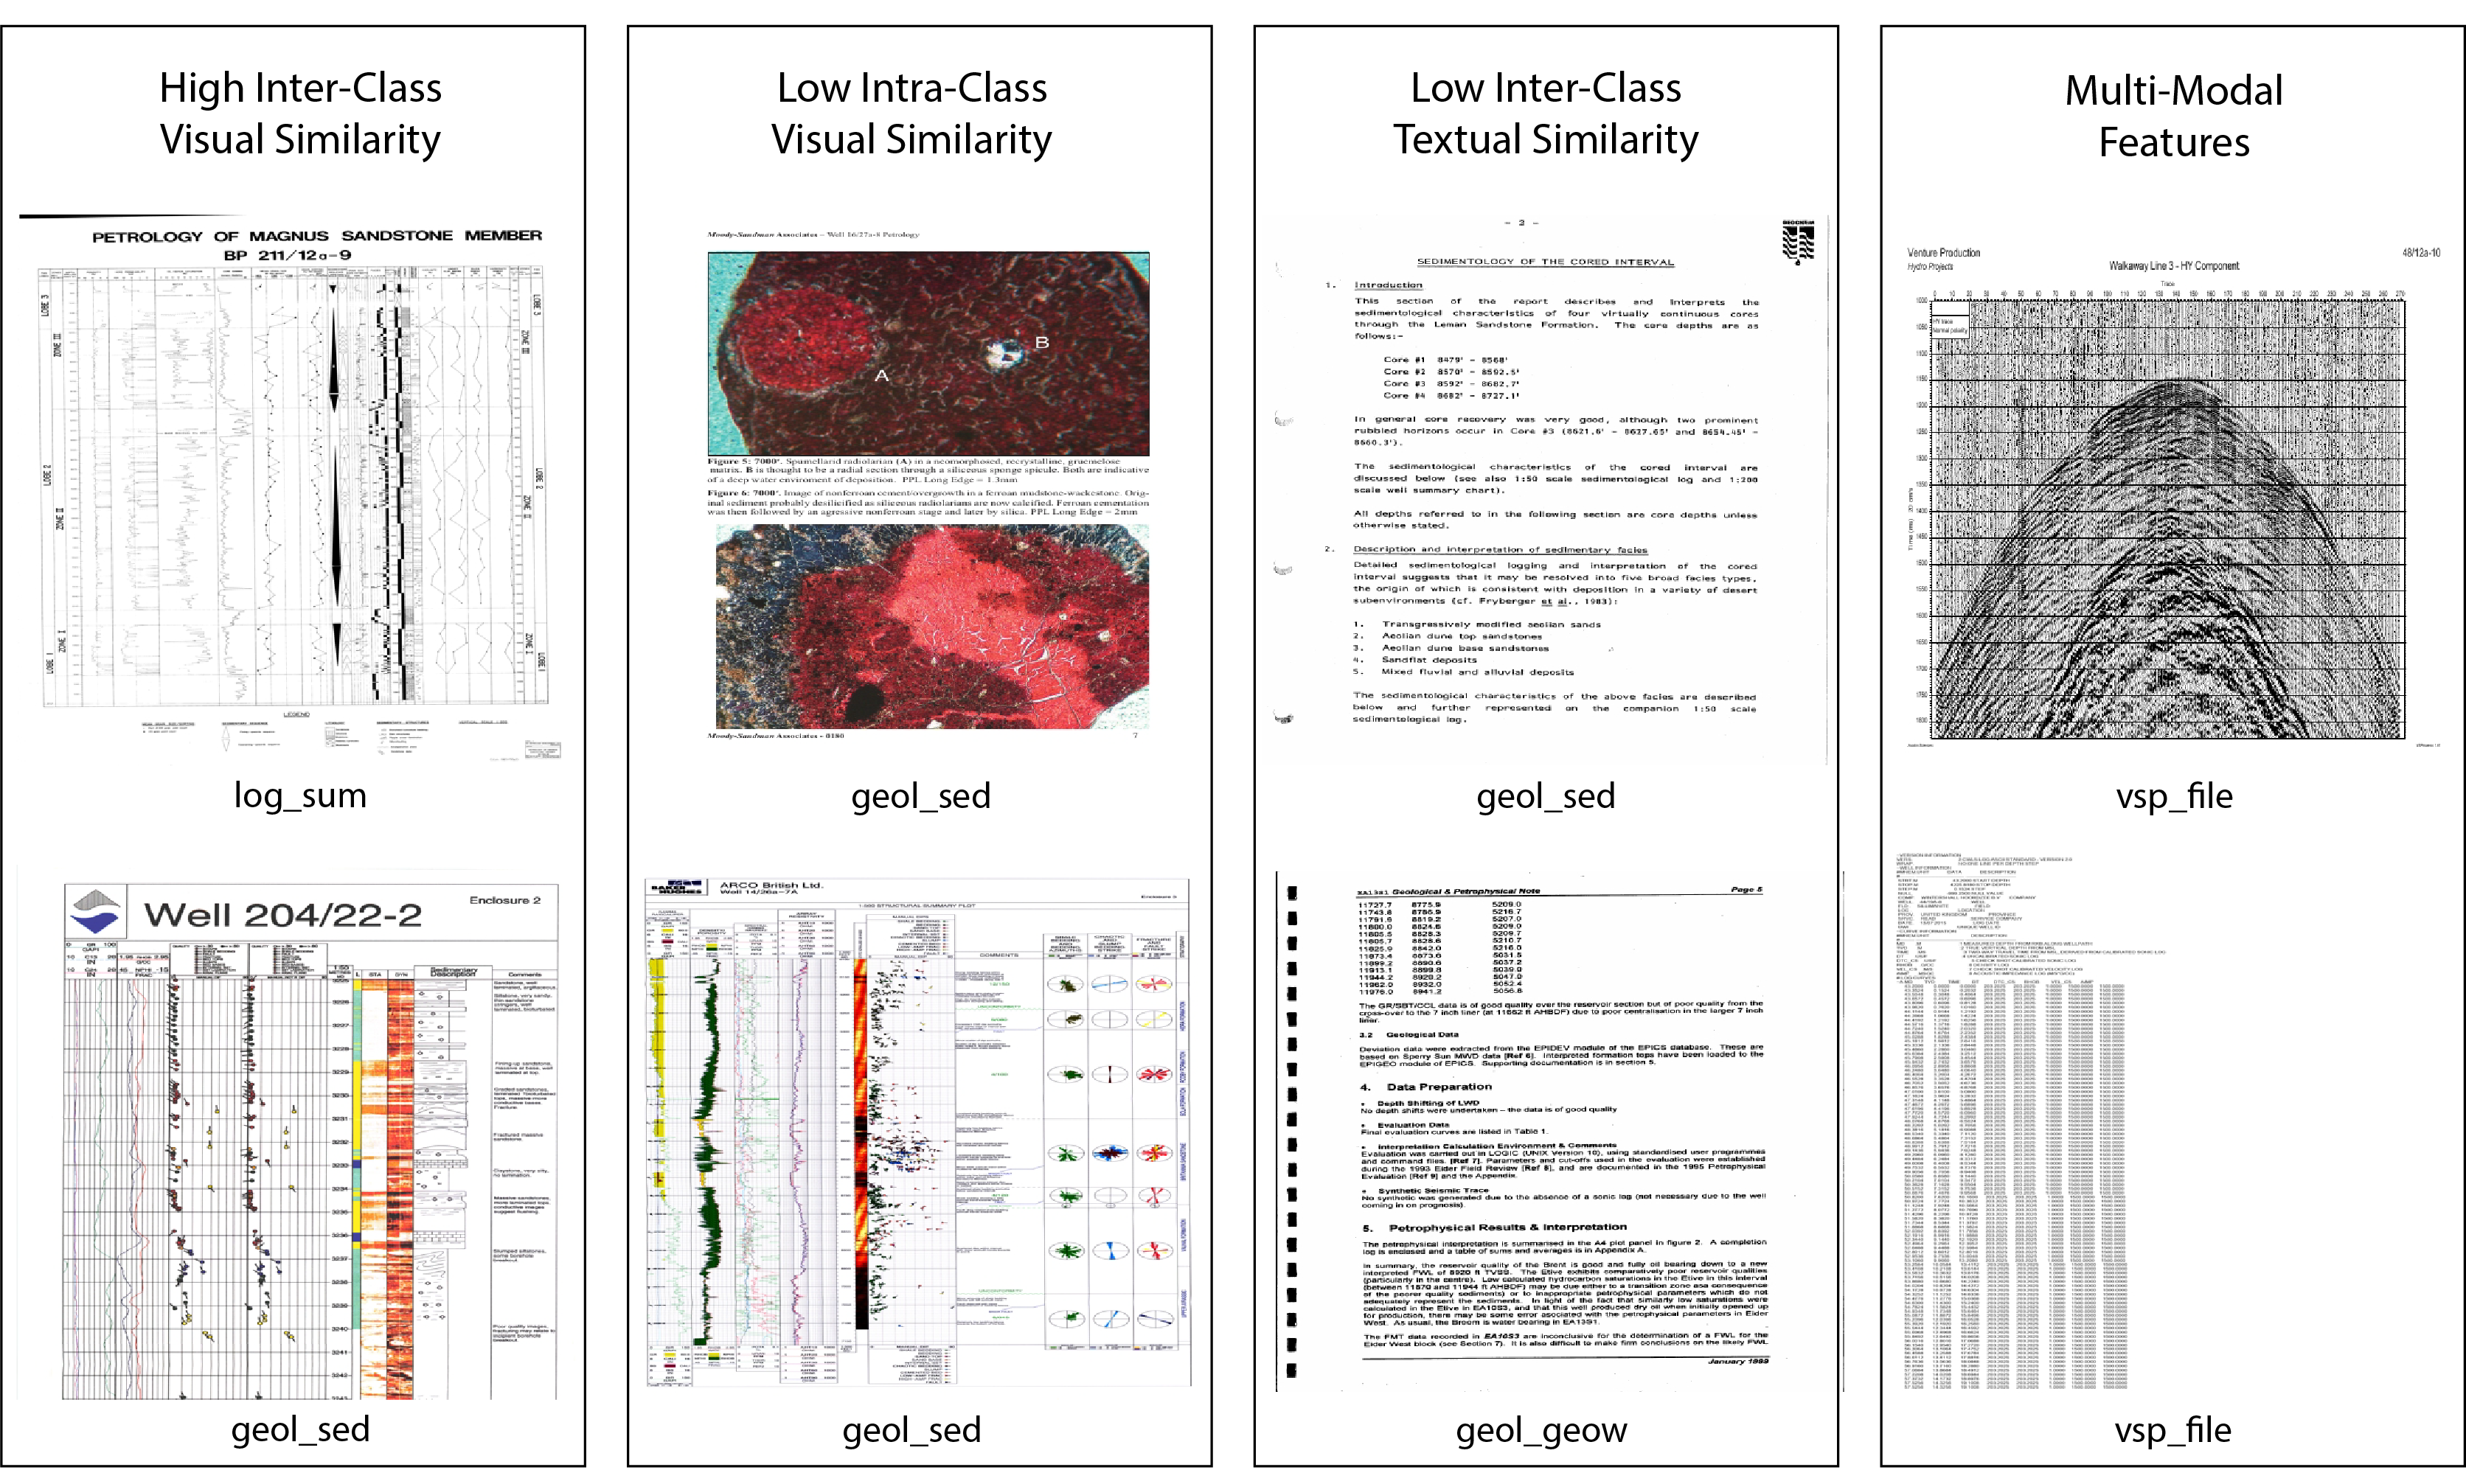
\includegraphics[scale=0.48]{page_samples.png}
\centering
\end{figure}

Contemporary uni-modal document classification models used in the industry often rely on features from a single modality, either textual or visual. However, it is difficult to build a robust high performance uni-modal classifier over such a complex multi-modal dataset. For example, document classifiers making use of visual features extracted from page images may underperform due to the high inter-class similarity or intra-class variance of some document page images.\\

The first column in Figure 1. shows an example of page images with high visual inter-class similarity, these are images representing different types of measurement logs which appear to be visually similar but are very distinct in the text modality. The second column shows an example of page images with low intra-class similarity, both are pages from geological sedimentary reports however both are visually very dissimilar. A final example of the text modality containing more useful information for classification are the visually indistinct plain text pages in column three. \\

Document classifiers that rely on features from only the text modality tend to outperform image based classifiers at classifying oil and gas documents at a granular level. However these classifiers only perform well when enough text data is present in a document, some documents in the corpus such as diagrams and sample images do not contain any text making them impossible to classify using a text based approach alone. Other documents contain very little text, that may be repeated across multiple document types. For example an oil well name and location being the only text data within visually different images such as between a map and a technical schematic. \\

This project proposes using a multi-modal approach to document classification, combining both text and visual modalities to create a more robust classifier for oil and gas exploration and production documents. Given heavy dependence on multi-modal communication of information and high cross-modal intra-class variability within these documents, it is possible to hypothesis that a multi-modal classification approach combining text and visual feature input streams, will outperform a classifier trained on features from a single modality such as text or visual features. \\

To investigate this, we will build on previous related work on multi-modal classification in other domains, applying and adapting these approaches to the classification of exploration and production documents. In particular we will investigate the various strategies for joining together both the text and visual modalities to give a single prediction, a process known as fusion. \\

\subsection{Related Work}
Baltrusaitis et al (2019) presented a survey detailing approaches to combining modalities for multimodal classification. The authors describe three different approaches to combining features from different modalities to make a classification decision, defining these as early, late and hybrid fusion. The early fusion method involves combing multi-modal features into a single representation prior to classification, whereas late fusion combines the output of two uni-modal classifiers to make a classification decision. The hybrid approach combines both the output of both early fusion and uni-modal classifiers to reach a classification decision. The survey also references Multiple Kernel Learning and Artificial Neural Networks (ANNs) as the types of models most commonly used in multi-modal learning.\\

Gallo et al (2018) proposed a multi-modal classification model using an early fusion technique, embedding encoded text visually onto an image prior to classification. The text is encoded using a one dimensional convolutional neural network (CNN) (Kim, 2014) and transformed into an encoded image. This is then superimposed onto the original image, which is then used as input to a CNN classifier. They concluded that this early fusion based approach out performed an identical CNN trained on uni-modal text and image inputs.\\

Audebert et al (2019) proposed a classification model with a late fusion architecture, merging the modalities in semantic space at decision time. For image classification a CNN with a MobileNetV2 architecture pre-trained against the ImageNet dataset was used. For text classification FastText  embeddings were used as input to a one dimensional CNN. The output of both the image and text classifiers was then flattened and fused by a single fully connected layer, with a final output softmax layer providing a classification prediction. Concluding that their late fusion model outperformed uni-modal classifiers when evaluated against the Tobacco3482 dataset and performed strongly against the RVL-CDIP dataset.  \\

Wang et al (2017) suggested that using a hybrid fusion based approach can improve text aided image classification performance. In this approach features for images were created using a pre-trained sixteen layer CNN, with text features consisting of dense embeddings generated using a two layer, one dimensional CNN (Milkov, 2013). Two separate softmax classifiers were then trained on the image and text features. Early fusion was achieved by learning shared image and text features, by concatenating the input features as inputs to a two layer feed forward neural network to train a third softmax classifier. The softmax output of these classifiers is then combined using late adaptive multimodal fusion to give the final classification result.\\

\section{Data Pre-Processing}
\subsection{Dataset Description}
The document corpus for this project comes from the National Data Repository (NDR), an online repository maintained by the UK Oil and Gas Authority for the storage of petroleum related information and samples. The NDR contains hundreds of thousands of documents, representing 65 document types defined by labels known as CS8 Codes. These are analogous to the key document types used internally by oil companies and therefore provide a good analogy for building a representative classification model for document retrieval across the industry. \\

There are several other well known document image datasets used for training and benchmarking models in the document analysis community. Many are derived from the Truth Tobacco Industry document corpus including the Tobacco-800 dataset, which contains 1,290 grayscale page images (Lewis, 2006), the Tobacco-3482 dataset which contains 3,482 grayscale page images (Kumar, 2013), the RVL-CDIP dataset consists of 400,000 grayscale images of document pages over sixteen classes (Harley, 2015). Unfortunately the use of a new oil and gas industry specific NDR dataset means we can't easily benchmark our models alongside other work, however it is hoped that sharing the extracted page images and text from the NDR corpus will enable further work both within the industry and the wider community.\\

For the purposes of this study, a document corpus was created by taking a random sample of approximately 1000 documents from each of 6 key document classes present in the NDR, with each document's provided CS8 Code being used as a classification label. The document classes (CS8 Codes) selected for inclusion in this dataset were; geological end of well reports (geol\_geow), geological sedimentary reports (geol\_sed), general geophysical reports (gphys\_gen), well log summaries (log\_sum), pre-site reports (pre\_site) and  vertical seismic profile files (vsp\_file).\\

\subsection{Feature Extraction}

As this is a new dataset, the text and page image features needed to be extracted from each document in the NDR corpus, for use as training, validation and test data for evaluating each of the classification models. The raw documents were downloaded manually via the NDR website and processed using a feature extraction pipeline written in Python 3.7 that calls the third party Apache Tika Server, Tesseract and Poppler libraries. \\

The extracted features from each document were saved to disk to create a persistent dataset, text features from each document were stored as a JSON file, while page image features were stored as a directory of JPEG files. The feature extraction process for each document was logged and stored as a row in a MySQL database table that maintained the relationship between each document and it's extracted feature files, recorded extraction status and tracked any errors encountered during the extraction process. \\

To make the feature extraction process efficient, the native Python multi-processing module was used to parallelise the workload into separate processes distributed across ten logical CPU cores. With each process extracting features from individual documents, supplied one at a time to each process via a shared queue and maintaining it's own database connection to track the extraction process.\\

Unfortunately features were not successfully extracted from all documents, some older Microsoft Office documents could not be processed, while others were corrupt or had non-standard file formats. Several documents also did not contain any text content and therefore lack a text feature set. A breakdown of the features available for each document class is provided in Table 1.\\

\begin{table}[H]
	\centering
	\begin{tabular}{| c | c | c | c |}
	\hline
	&\textbf{Extracted} & \textbf{Extracted} & \textbf{Either}\\
	\textbf{Document Class} & \textbf{Image Features} & \textbf{Text Features} & \textbf{Features}\\
	\hline
	geol\_geow & 1609 & 1477 & 1609\\
	\hline
	geol\_sed & 1013 & 964 & 1013 \\
	\hline
	gphys\_gen & 1041 & 876 & 1041 \\
	\hline
	log\_sum & 1051 & 887 & 1051\\
	\hline
	pre\_site & 1154 & 1053 & 1154\\
	\hline
	vsp\_file & 673 & 621 & 673\\
	\hline
	\textbf{Total:} & \textbf{6541} & \textbf{5878} & \textbf{6541}\\
	\hline
	\end{tabular}
	\caption{\label{tab:table-name}Count of Feature Sets Extracted per Document.}
\end{table}

\subsection{Text Pre-Processing}
The text feature dataset consists of a vector of integers $T$ for each document representing the first 2,000 informative terms following text extraction and pre-processing. To create each vector, each document's text first had to be extracted. Text extraction from ascii format files was achieved using native Python, for scanned PDF files without an embedded text layer and image format files, text was extracted using the Tesseract OCR Engine (Smith, 2007). Some PDF format files in the corpus contain an embedded searchable text layer, these are usually PDF files that have been digitally created or that have previously undergone OCR as part of a digitisation project, text from these files was extracted using Apache Tika Server (Tiedemann, 2014).  \\

The raw text extracted from each document was case folded to lower case and tokenized using the pre-trained Word Punkt tokenizer (Kiss, 2006) available in the NLTK library, into a sequence of individual tokens. Any tokens with low semantic value were then dropped from the sequence, including non-word tokens such as numbers and punctuation, as well as frequently occurring stopwords. Each token was then lemmatized to it's base form using the Word Net (Miller, 1995) lemmatizer in NLTK, this reduces dimensionality while preserving the semantic meaning of each token term.\\

The processed tokens were then converted to integers, this was achieved by creating a vocabulary set $V$ containing all unique tokens extracted from each document and mapping each to a unique integer value $v$. The first 2,000 processed tokens for each document are then mapped to their corresponding $v$ integer value in $V$ to create a vector of integers $T$ for each document. Any vectors with less than 2,000 integers are padded with 0 so that $|T| = 2,000$ giving a consistent input size for our models.\\

\subsection{Image Pre-Processing}
The visual feature dataset consists of sequences of JPEG images, with each sequence $S$ representing the first ten pages of each document in the corpus. For documents in a non-image file format the pages were converted to image representations. For PDF format documents each page was converted to a single JPEG image using the Poppler PDF rendering library, for raw text format files a new blank image with all white pixels was created using a standard A4 page size of 1748 x 2480 pixels and the documents text content was fitted to and overlayed on each blank page image. For documents with less than ten pages, each sequence was then padded with blank 2D arrays with all pixel values in each array set to zero so $|S| = 10$. \\

Each extracted page image was then resized to 200 x 200 pixels using cubic interpolation to make them small enough to be fed into the classification CNN. This size has been selected as a compromise between the loss of information in the image verses the computational cost of a larger image size, as well as a desire for a consistent input size for our models. Larger input sizes may also lead to overfitting as the CNN may learn more granular features such as characters or image details that are only relevant to specific documents in the training dataset, instead of the overall general layout of documents within a class (Kang, 2014).\\

Certain documents within the corpus have pages with very large aspect ratios, documents in the comp\_log class for example often have a vertical aspect ratio of c. 12.0 compared to the aspect ratio of 1.414 of a typical A4 document page. Resizing these images to 200 x 200 pixels causes significant loss of layout and image information. Therefore, page images with an aspect ratio greater than 2.0 were split into multiple consecutive images, each with an aspect ratio of 1.414 prior to being resized, with each image being treated as a separate page in the document.\\

To further reduce unnecessary complexity the page images were converted to single channel greyscale format using Floyd-Steinberg dither to approximate the original image luminosity levels (Floyd, 1976), the original RGB format images were also tested but when benchmarked against the uni-modal image classification model the accuracy gains were not significant and had a significant computational cost. As a final pre-processing step the pixel values in each page image were normalized by dividing each pixel value by the maximum intensity value of 255.

\section{Experiment Design}
\subsection{Experiment Goals}
In this work we seek to investigate the effectiveness of multi-modal deep learning at the task of classifying the multi-page documents within the NDR corpus. First in order to provide a benchmark against which to measure the performance of the multi-modal models two uni-modal models will be evaluated, a text based classifier and a classifier built using page images. Various multi-modal approaches that combine both document text and page images will then be explored using early, late and combined fusion architectures. \\

\subsection{Model Hyperparameters}
The majority of hyperparameters will be specific to each model architecture used in this work, however a number of hyperparameters are fixed for all models. This makes comparing the performance of the models easier and allows the combination of uni-modal model architectures into the more complex multi-modal models. Model specific parameters are adapted from previous work or determined experimentally and tunned using a grid search optimisation approach. \\

For the fixed hyperparameters the ReLU activation function is used for all hidden network layers, with a softmax activation function being used for all output layers. Every model also uses the Adam optimization algorithm (Diederik, 2014) to optimize a categorical cross entropy loss function, with the default TensorFlow learning rate of 0.001 providing a good balance of classification accuracy and performance when tested experimentally with various rates on both uni-modal models.\\

\subsection{Model Training}
The dataset used for training and evaluating each model will be split with 80\% being used for training and 20\% being used for testing model performance, with 10\% of the training dataset being set aside for use in validation during model training. The dataset is split randomly and in a stratified manner to ensure an even split across all classes, a random seed is used to ensure reproducibility.\\

To avoid overfitting the models due to over-training the training process is terminated using an early stopping technique. At the end of each training epoch the model's performance is measured against the validation set and if the validation loss has not decreased for two consecutive epochs, training is halted. The model weights are then reverted to the state with the lowest validation loss to produce the final trained model. Once training is complete each model will be evaluated using the same performance metrics; overall percentage accuracy, macro precision and recall scores, macro F1 score and the number of epochs each model takes to converge.

\subsection{Model Evaluation}
The first step in evaluating each model is the conversion of the class probability predictions provided by the softmax output layer into discrete classification predictions using an $argmax$ function. The models accuracy can then be calculated by dividing the count of correctly predicted classes by the count of all predictions, giving a measure of the models overall predictive performance.\\

The precision, recall and $F1$ performance scores are calculated using macro-averaging, as this treats all classes equally and performs well across balanced datasets (Sokolova, 2009). Macro precision ($precision_m$) is calculated as the ratio of documents correctly predicted ($TP$) in a class ($c$) to all documents predicted to be in that class ($TP + FP$) averaged over all classes. Whereas macro recall ($recall_m$) is the ratio between documents correctly predicted ($TP$) to be in a class ($c$) to all documents incorrectly predicted to belong to another class ($FN$), averaged over all classes. The macro $F1$ score is calculated as the harmonic mean of the $precision_m$ and $recall_m$ scores, this gives a measure of the balance between precision and recall placing equal importance on both. In the context of the NDR document classification task a good balance is ideal, therefore $F1$, $precision_m$ and $recall_m$ scores of near one are desirable.\\

\begin{center}
$precision_m = \dfrac{\sum_{i=1}^{c}TP_i\  /\ (TP_i + FP_i)}{6} $\\
\vspace{0.5cm}
$recall_m = \dfrac{\sum_{i=1}^{c}TP_i\   /\   (TP_i + FN_i)}{6} $\\
\vspace{0.5cm}
$F1_m = \dfrac{2 \times precision_m \times recall_m}{precision_m + recall_m} $\\
\end{center}
\vspace{0.5cm}

The stochastic nature of training a deep learning model also needs to be accounted for in the model evaluation process. A model with a set architecture can vary in performance due to a number of factors, including random weight and bias initialization values or the stochastic behaviour of the Adam optimisation algorithm as it traverses the error gradient. To compensate for the effect of model variance on the evaluation of model performance, each model is initialized and evaluated ten times with the average performance metrics of all ten initializations being taken as the models overall performance.\\

To measure how well the model generalises across the entire NDR dataset instead of simply optimising the model to predict a specific test sample, it is necessary to also vary the sub-samples used in training, validating and testing the model. Therefore a different random sample split is used for each iteration and to ensure the same sub-samples are used for each model a random seed $s$ for $s \in \{2020, 2021, 2022, 2023, 2024, 2025, 2026, 2027, 2028, 2029\}$ is used in sequence to calculate each iterations split values. When an average performance metric such as average accuracy is mentioned in this work, it can be assumed the metric has been calculated using this technique.\\

All models in this paper were built using the TensorFlow 2.3 framework in Python 3.7 and trained using GPU accelerated computing using CUDA 10.1 with an Nvidea RTX 2070 SUPER GPU.

\section{Baseline Models}

\subsection{Text Classification Model}
The text classification model used in this project is based on the simple 1D CNN model for text classification first proposed by Kim (Kim, 2014). The original model had a simple architecture with just a single convolutional layer, followed by a global max pooling layer and a fully connected softmax output layer. To avoid overfitting or co-adaptation of hidden units, dropout is employed in the penultimate network layer, reportedly improving the performance by up to 4\% (Kim, 2014). An $l2$ norm constraint is also applied to help further regularise the model.\\

The original model made use of pre-trained Word2Vec word embeddings trained on a 100 billion word Google News corpus using the continuous bag of words (CBOW) method (Mikolov, 2013) as inputs, these dense embeddings attempt to capture the semantic and syntactic meaning of each word in the training corpus and have been shown to perform better than sparse representations such as TF-IDF or one hot encoding in text classification tasks.\\

Unfortunately generic pre-trained neural language models struggle to capture domain specific semantics and vocabulary, resulting in a  large number of out of vocabulary terms (Sarma, 2018). Therefore the generic Word2Vec model does not perform well for the classification of corpora with highly domain specific vocabularies, such as in the oil and gas industry specific NDR corpus (Sarma, 2018). With this in mind the text classification model makes use of bespoke dense embeddings, learned during training through the use of an embedding layer. The embedding layer is initialized with random weights, which are then updated during training to learn dense word embeddings, each with a vector length of 150 values. This approach has the advantage of learning embeddings specific to the classification task and corpus texts, however due to the more limited training set, these embeddings are likely to be of lower quality.\\

Despite having a relatively simple architecture, originally proposed for the classification of shorter sentences, this model has been shown to be very effective against well know document classification benchmark datasets. However hyperparameter tunning of the original model is required to maximise classification performance. As a baseline the model was initially fitted and tested using the original architecture and hyperparameters as shown in Table 2. with the bespoke embedding layer discussed above. When trained with the original hyperparameters the model converged after an average of 23 epochs, the trained model had an average accuracy of 82.6\%, average recall score of 0.83, average precision score of 0.83 and an average macro f1 score of 0.83 when evaluated against the test dataset.\\

\begin{table}[H]
	\centering
	\begin{tabular}{| c | c | c |}
	\hline
	&&\\
	\textbf{Hyperparameter} & \textbf{Original Model} & \textbf{Tunned Model}\\
	\hline
	Kernel Size & 4 & 7\\
	\hline
	Feature Maps & 100 & 200\\
	\hline
	Activation Function & ReLU & ReLU\\
	\hline
	Pooling & Global 1-Max Pooling & Global 1-Max Pooling\\
	\hline
	Dropout Rate & 0.5 & 0.3 \\
	\hline
	$l2$ Regularisation & 3 & 0.5\\
	\hline
	Dense Hidden Layers & 0 & 1\\
	\hline
	Dense Layer Nodes & 0 & 50\\
	\hline
	\end{tabular}
	\caption{\label{tab:table-name}Hyperparameters of Original (Zhang, 2017) and Tunned Model.}
\end{table}

The model was then optimised for the task of classifying documents in the NDR corpus through hyperparameter tuning. A coarse grid search was performed on each of the following hyperparameters to find it's optimal values relating to the models classification performance; the kernel size of each feature region and the number of feature maps in the convolutional layer, the dropout rate and the $l2$ norm constraint threshold.\\

The range of value sets used in the grid search were taken from a previous study that examined empirically across a number of corpora, which hyperparameters are most important to tune to improve the performance of the original sentence classification model (Zhang, 2017). During the grid search procedure each hyperparameter is tunned separately and  all other parameters, weights and biases are kept constant, the highest performing value is selected for the final model.\\

\begin{table}[H]
	\centering
	\begin{tabular}{ r l c  c }
	Kernel Sizes & $= \ \{1, 3, 5, 7, 10\}$\\
	Feature Maps &= \ $\{10, 50, 100, 200, 400, 600\}$\\
	Dropout Rate &= \ $\{0.1, 0.2, 0.3, 0.4, 0.5\}$\\
	$l2$ Norm Constraint &= \ $\{0.5, 1, 2, 3\}$\\
	\end{tabular}
	\caption{\label{tab:table-name}Hyperparameter Ranges (Zhang, 2017).}
\end{table}

We also experimented with adding dense feed forward layers prior to the dropout and softmax output layers, finding that the addition of a single fully connected feed forward layer improved model performance while reducing the number of epochs taken for the model to converge. A coarse grid search was conducted using different numbers of nodes $n \in \{ 50, 100, 250, 500, 1000 \}$ in the dense fully connected layer, finding 50 nodes to be optimal. Varying the number of convolutional layers in the model was also tested, as deeper architectures have been shown to be highly effective at text classification tasks. However in this case adding additional convolutional layers had a high computational cost and did not significantly improve model performance.\\

The optimal hyperparameters identified for the tunned model are shown in Table 2. Once trained with these hyperparameters the tunned model yielded an average test accuracy of 86.3\%, an improvement of 3.7\% compared to the original model. The model also had an improved average macro $F1$ score of 0.86. Obviously given that this model has been trained and evaluated against only documents which contained text data, when the evaluation metrics are extended to include all documents in the NDR corpus the text based approach has an average macro accuracy of 77.7\%.

\subsection{Page Image Classification Model}
Two dimensional CNNs have revolutionised deep learning performance in the area of image classification, including the classification of document page images (Kang, 2014). Most prior work in document classification has focused on the use of CNNs to classify documents one page at a time as a continuous document stream of discrete page images (Wiedemann, 2018). We attempt to replicate previous work in this area by first evaluating a single page CNN classifier on only the first page, then expanding this approach to multi-page document classification. \\

We then build on this work, evaluating a combined C-LSTM (Convolutional Long Short Term Memory) architecture that takes the original CNN network and places it within an LSTM network architecture to classify documents based on their entire page image sequences. LSTM networks are a form of recurrent neural network capable of learning temporal relationships between the page images such as page order and proximity. We hypothesize that this approach will perform better on the NDR document classification task, factoring the composition and order of multiple pages into a documents classification. It is our hypothesis that this approach will perform better on the NDR classification task, in part by helping overcome the high intra-class similarity of some individual page images. \\

The single page CNN model architecture was adapted from previous work on page image classification (Kang, 2014), in which greyscale document page images similar to those in the NDR dataset were classified with an overall accuracy of 65.35\%. The models architecture consists of two convolutional layers, and two max pooling layers, the output of which is fed into a two layer dense feed forward network with 1000 nodes in each layer, followed by a final softmax output layer. The first convolutional layer has 20 feature maps and kernel size of 7 x 7, the second convolutional layer has 50 feature maps and a kernel size of 5 x 5, both max pooling layers have 4 x 4 pooling kernels. The network is regulated by applying dropout at the penultimate layer at a rate of 0.5, this masks out the output activations from 50\% of the neurons in the final dense layer. The model was tested with each dropout rate $ r \in \{0, 0.1, 0.2, 0.3, 0.4, 0.5, 0.6\}$ with the optimal dropout rate being 0.5 as per the original paper. The variation of other model hyperparameters was tested, however the only change made that improved the performance of the original model was the use of zero padding on the output of the initial convolutional layer. \\

We then expanded the use of the single page CNN architecture to multi-page document classification. First an ensemble approach was tested with the majority vote being taken as a documents class, with the strength of the softmax probability prediction being used to resolve any conflicts. First the single page CNN model was trained on all ten pages from every document. The model was able to classify individual pages with an accuracy of 49\% and $F1$ score of 0.48. During model evaluation, inference was performed on all pages in a document using the majority vote method to give a final prediction for the document as a whole. Unfortunately this approach performed poorly with an accuracy of 50\%, which may be in part due to the model trying to classify zero padding images in the input sequence. \\

Following the poor performance of the majority vote approach the use of a simple neural network classifier was investigated to combine the output probabilities for each page into a single document classification (Ju, 2017). The theory behind trying this approach was that even a simple neural network should be able to learn to place less value on zero value padding images and similar pages across classes, while recognising meaningful class specific pages or probability combinations. The CNN output probabilities for each page were concatenated into a single feature vector and used as input to a simple three layer neural network classifier. The classifier architecture consisted of a 60 node input layer, a hidden 10 node fully connected layer and a 6 node softmax output layer, with the number of nodes in the hidden layer being determined by a grid search of $n \in \{  5, 10, 15, 20, 30 \}$. When evaluated this approach gave a classification accuracy score of 72.4\% a major improvement of 22.4\% compared to the majority vote method and a significant accuracy improvement of 5.3\% over the Single Page CNN. \\

The use of a C-LSTM model architecture was then investigated, with the aim of unifying multi-page classification into a single model that can learn important temporal relationships within document page sequences. The C-LSTM model uses the same CNN architecture as the single page model as time distributed feature extractors. The output sequence from the temporal CNN feature extraction layers is then fed into two uni-directional LSTM layers in place of the previous dense layers used in the Single Page CNN. The output of the final CNN layer is regulated using dropout prior to the final softmax output layer. The optimal number of nodes in the LSTM layer $n$ and dropout rate $d$ were determined using grid search for $n \in \{250, 400, 450, 500, 550, 600, 750, 1000\}$ and $d \in \{0.1, 0.2, 0.3, 0.4, 0.5\}$  with $n$ = 1000 and $d$ = 0.5 giving optimum model performance. The C-LSTM model performed significantly better than the Single Page CNN, showing an improvement of 6.5\% average accuracy. How ever it performed  worse than the Multi-Page CNN with the additional neural network ensemble layer, which had a 1.1\% higher accuracy. However this is only a marginal gain with the simpler single model architecture and faster inference making the C-LSTM a more practical choice. The use of bi-directional LSTM layers in place of the uni-directional LSTM layers was also evaluated but did not improve the average performance of the model. An overview of average performance metrics for each page image classification model has been provided in Table 4.

\begin{table}[H]
	\centering
	\resizebox{\textwidth}{!}{%
	\begin{tabular}{ | c | c c c c c | }
	\hline	
	\textbf{Model} &  &  & \textbf{Average} &  & \\
	\textbf{Architecture} & \textbf{Accuracy} & \textbf{Precision} & \textbf{Recall} & \textbf{$F1$ Score} & \textbf{Epochs}\\
	\hline
	Single Page CNN &&&&&\\
	(First Page) & 67.1 \%& 0.69 & 0.68 & 0.68 & 4 \\
	\hline
	Multi-Page CNN &&&&&\\
	(Majority Vote) & 44.8 \%& 0.59  & 0.42  & 0.40  &  \textbf{3} \\
	\hline
	Multi-Page &&&&&\\
	CNN (NN) & \textbf{72.4 \%}& \textbf{0.75} & \textbf{0.73} & \textbf{0.73} & 3 + 7 \\
	\hline
	Uni-Directional &&&&&\\
	C-LSTM & 71.3 \% & 0.74 & 0.72 & 0.72 & 8 \\
	\hline
	Bi-Directional  &&&&&\\
	C-LSTM & 70.3 \% & 0.73 & 0.71 & 0.71 & 6 \\
	\hline
	\end{tabular}}
	\caption{\label{tab:table-name}Uni-Modal Page Image Classifier Performance.}
\end{table}

\section{Multi-Modal Models}

\subsection{Early Fusion Model}
Early fusion in multi-modal deep learning involves the early concatenation of uni-modal features, usually immediately after feature extraction into a single joint representation (Baltrusaitis, 2018). In deep neural network classifiers this single joint representation is then used as input to the models decision layers. The early combination of modalities prior to classification, allows the model to learn important inter-modal features and low level correlations across both modalities (Gao, 2020). This approach is loosely analogous to how biological neural networks perform multisensory convergence early on in their sensory processing pathways (Schroeder, 2005). However an early fusion model is less likely to learn strong modality specific features than models using late or hybrid fusion, which may hamper classification performance when one of the text or image modalities is missing. \\

The architecture of the early fusion neural network used for this experiment is a C-LSTM that concatenates the page image and text features post extraction to provide a joint representation. Feature extraction for each modality is initially performed separately, using an identical approach to feature extraction as that used in the previously evaluated uni-modal networks. A one-dimensional CNN, with word embeddings and a global max-pooling layer is used to extract features from the input text. A dual layer two-dimensional CNN is used to extract features from the input page images, consisting of alternating convolutional and max pooling layers. The extracted features from both are then flattened and concatenated into a joint feature representation, this is then fed into two LSTM cell layers followed by a single softmax layer that provides the classification prediction probabilities. \\

As in the uni-modal page image classification C-LSTM model a recurrent LSTM architecture is used to allow the model to learn important temporal relationships between the page images, however the LSTM cell layers require inputs to be a time distributed sequence. The image inputs already exist in an ordered sequence of ten pages and distributing them as inputs is trivial, however there is only a single instance of text input data per document. Therefore to create a joint feature representation that can be processed by the LSTM, the text data is replicated ten times to create a sequence of ten identical texts. This allows features from each page image to be concatenated with those from the documents extracted text and processed by the LSTM as a single temporally distributed joint sequence.\\

Due to the time and space complexity of the model as well as the large number of tuneable parameters, it was unfeasible to use grid-search or even Bayesian hyperparameter optimisation methods on all layers and parameters of the network. Therefore hyperparameter tunning was only carried out on the final LSTM and regularisation layers, making the assumption that the feature extraction layers have already been optimised for feature extraction on the input data during the tunning of the uni-modal models. A coarse grid search was performed on a per feature basis, exploring the number of nodes $n = \{250, 400, 450, 500, 550, 600, 750, 1000\} $ in each LSTM layer and the dropout rate applied to regulate the model at the penultimate layer $d = \{ 0.1, 0.2, 0.3, 0.4, 0.5, 0.6 \} $. This process identified 1000 nodes and a dropout rate of 0.5 was optimal for the final LSTM layer, interestingly creating a bottleneck by using only 450 nodes in the first LSTM layer led to a reasonable increase in classification performance. The addition of a dense fully connected layer between the final LSTM and softmax output layer was also tested with varying numbers of nodes, however this layers addition was found to degrade the models performance. The final high level architecture for the early fusion model is shown in Figure 2. \\

\begin{figure}[H]
\caption{Early Fusion Model Architecture}
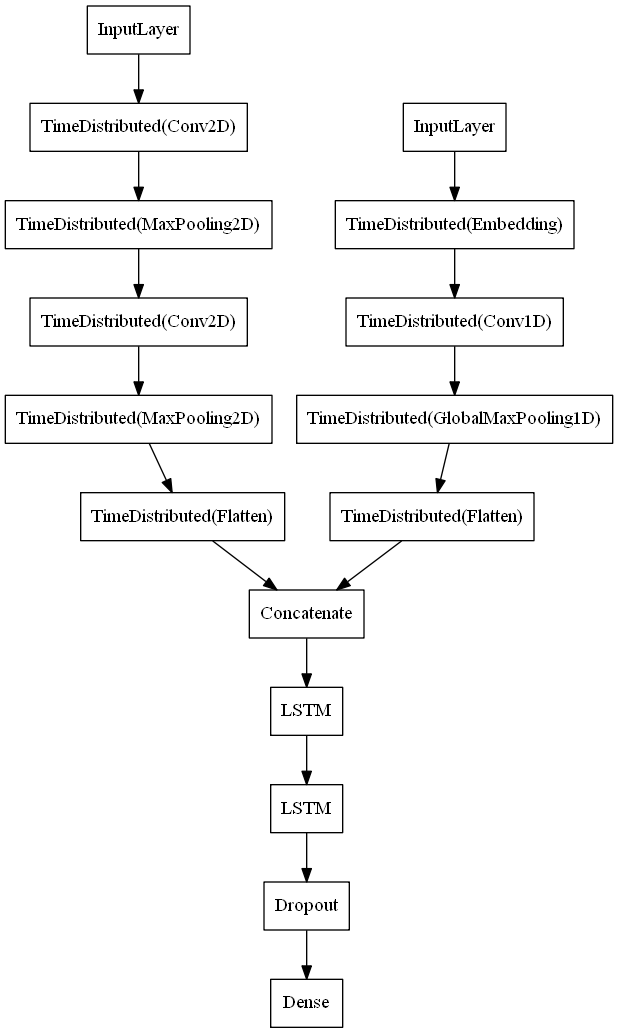
\includegraphics[scale=0.35]{early_fusion_model.png}
\centering
\end{figure}

\subsection{Late Fusion Model}
The late fusion method makes use of two separate uni-modal networks and fuses their semantic output representations at decision time (Hossain, 2010). Each uni-modal network performs feature extraction and learns strong modality specific representations for use in document classification, the output of the final layer of each uni-modal network is then fused to give a join classification decision. This approach in theory allows the model to be more robust to missing data from one modality.\\

There are a number of approaches to late fusion in deep neural classifier networks, in some approaches the uni-modal networks are trained separately, then their free parameters are frozen and the output of their penultimate layers fused together by a dense fully connected output layer. The approach taken for our late fusion model is similar, however the weights and biases in the uni-modal models are not frozen and trained together as part of a multi-modal network.\\

The late fusion model was constructed by taking the architectures of the uni-modal 1D text classification CNN and uni-directional C-LSTM page image sequence classification models and replacing their output layers with a single shared six node softmax output layer. Each uni-modal network is otherwise left unchanged, with the same layers, regularisation and other hyperparameters as the original models. The final high level architecture for the late fusion model is shown in Figure 3. \\

\begin{figure}[H]
\caption{Late Fusion Model Architecture}
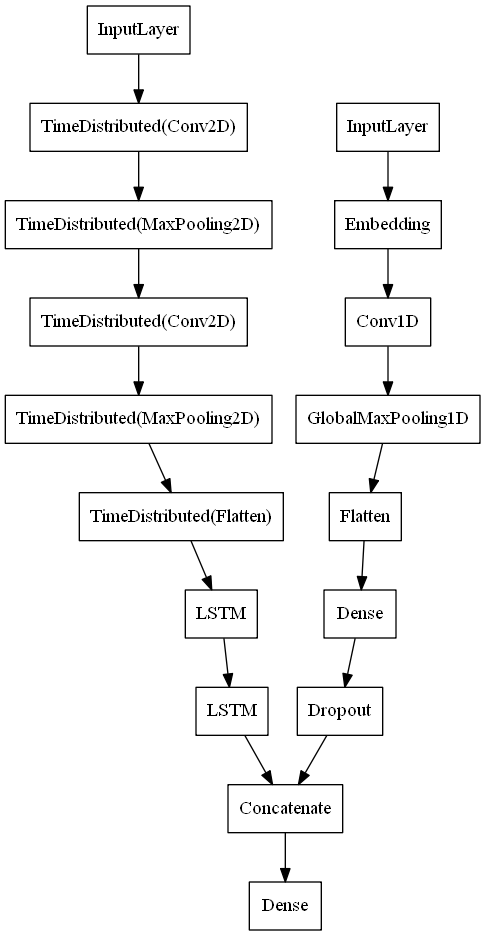
\includegraphics[scale=0.35]{late_fusion_model.png}
\centering
\end{figure}

\subsection{Hybrid Fusion Model}
Hybrid fusion networks attempt to combine the benefits of the early and late fusion strategies, with the goal of creating a model that can learn both strong feature and decision level strategies (Atrey, 2010). The hybrid model used in this experiment combines the architectures of the previous early and late fusion models, concatenating the penultimate layers into a single representation connected to a softmax output layer. The final high level architecture for the hybrid fusion model is shown in Figure 4.\\

\begin{figure}[H]
\caption{Hybrid Fusion Model Architecture}
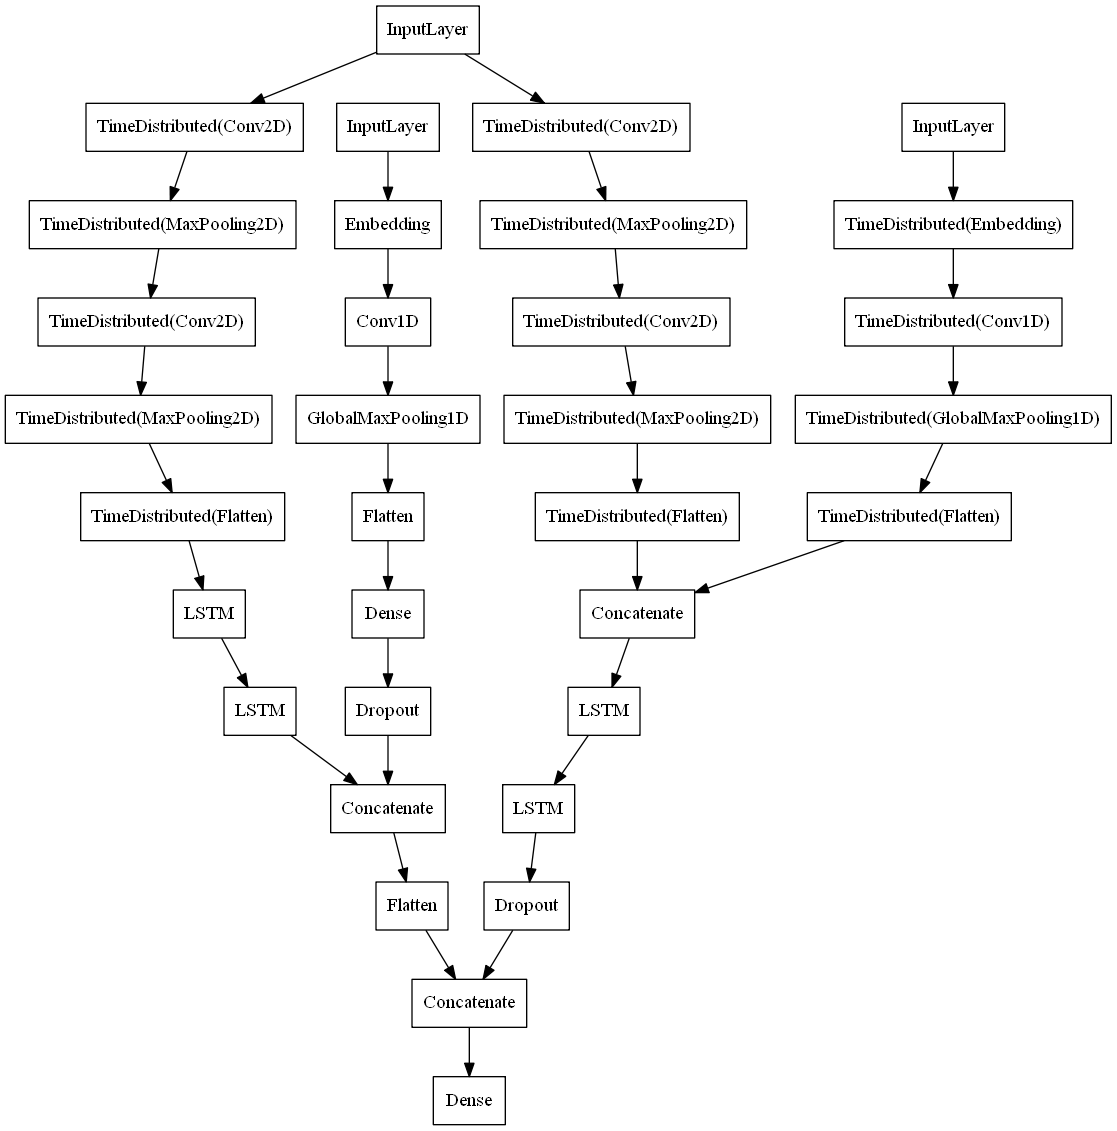
\includegraphics[scale=0.35]{hybrid_fusion_model.png}
\centering
\end{figure}

\section{Evaluation}

\subsection{Model Benchmarking}
To assess the average classification performance of the different fusion strategies, each of the fused models were trained and benchmarked against two datasets from the NDR corpus. To measure general performance and allow for benchmarking against the uni-modal text classification model, each multi-modal model was benchmarked against a sub-set of the NDR in which all documents contained both page image and text features, this will from now on be referred to as the Dual Modality Dataset. The benchmark performance metrics for each multi-modal model on this dataset are provided in Table 5.\\

Then to measure the robustness of the models in classifying documents that lack any text data, each model was also trained and benchmarked against the entire NDR corpus, we will refer to this as the Complete Dataset. This allows any loss in classifier performance due to a uni-modal image only input to be quantified, as well as allowing the multi-modal models to be benchmarked against the uni-modal image classification CNN model. It's worth noting that robustness to this type of input is is an important performance benchmark as documents that lack text data are common in the NDR corpus and the wider Oil and Gas industry, examples of these document types include microscopy images, seismic profiles and some maps. The benchmark performance metrics for each multi-modal model on the Complete Dataset are provided in Table 6.\\\\

To measure if the performance difference between similarly performing models is statistically significant the Wilcoxon signed-rank test is used to calculate a p-value. This test has been selected as it is more robust to the non-independence of performance values caused by the random resampling approach used to evaluate each model multiple times across the dataset and does not assume homogeneity of variance (Demšar, 2006). This allows us to test the null hypothesis that the difference in performance between to models may be due to random chance, we can reject this hypothesis if the score is below the widely used threshold of 0.05.   \\
\begin{table}[H]
	\centering

	\begin{tabular}{ | c | c | c c c c |}
	\hline
	\textbf{Model} & \textbf{Seed} & \textbf{Accuracy} & \textbf{Precision} & \textbf{Recall} & \textbf{F1 Score}\\
	\hline	
	& 2020 & 79.6 \% & 0.82 & 0.78 & 0.79\\
	& 2021 & 80.7 \% & 0.82 & 0.81 & 0.81\\
	& 2022 & 84.4 \% & 0.85 & 0.85 & 0.84\\
	Early & 2023 & 85.6 \% & 0.86 & 0.76 & 0.86\\
	Fusion & 2024 & 80.7 \% & 0.81 & 0.81 & 0.80\\
	C-LSTM & 2025 & 84.2 \% & 0.85 & 0.85 & 0.85\\
	& 2026 & 81.9 \% & 0.85 & 0.81 & 0.82\\
	& 2027 & 83 \% & 0.80 & 0.79 & 0.79\\
	& 2028 & 84.5 \% & 0.85 & 0.84 & 0.84\\
	& 2029 & 77.2 \% & 0.85 & 0.85& 0.85\\
	\hline
	\multicolumn{2}{| c |}{\textbf{Average}} & \textbf{82.5} \% & \textbf{0.84} & \textbf{0.83} & \textbf{0.83}\\
	\hline
	& 2020 & 83.3 \% & 0.83 & 0.83 & 0.83\\
	& 2021 & 84.3 \% & 0.85 & 0.85 & 0.85\\
	& 2022 & 82.4 \% & 0.83 & 0.84 & 0.83\\
	Late & 2023 & 86.4 \% & 0.87 & 0.87 & 0.87\\
	Fusion & 2024 & 85.5 \% & 0.85 & 0.85 & 0.85\\
	C-LSTM & 2025 & 84.5 \% & 0.86 & 0.85 & 0.85\\
	& 2026 & 83.6 \% & 0.85 & 0.84 & 0.84\\
	& 2027 & 84.8 \% & 0.85 & 0.84 & 0.85\\
	& 2028 & 84.2 \% & 0.85 & 0.85 & 0.85\\
	& 2029 & 82.7 \% & 0.84 & 0.83 & 0.73\\
	\hline
	\multicolumn{2}{| c |}{\textbf{Average}} & \textbf{84.2} \% & \textbf{0.85} & \textbf{0.85} & \textbf{0.85}\\
	\hline
	& 2020 & 83.4 \% & 0.85 & 0.84 & 0.80\\
	& 2021 & 83.3 \% & 0.85 & 0.84 & 0.77\\
	& 2022 & 83.1 \% & 0.84 & 0.83 & 0.78\\
	Hybrid & 2023 & 81.7 \% & 0.83 & 0.82 & 0.75\\
	Fusion & 2024 & 81.3 \% & 0.82 & 0.81& 0.78\\
	C-LSTM & 2025 & 85.4 \% & 0.85 & 0.86 & 0.79\\
	& 2026 & 81.6 \% & 0.84 & 0.81 & 0.81\\
	& 2027 & 81.3 \% & 0.82 & 0.81 & 0.81\\
	& 2028 & 82.9 \% & 0.84 & 0.83 & 0.83\\
	& 2029 & 72.3 \% & 0.84 & 0.83 & 0.83\\
	\hline
	\multicolumn{2}{| c |}{\textbf{Average}} & \textbf{82.6} \% & \textbf{0.84} & \textbf{0.83} & \textbf{0.83}\\
	\hline

	\end{tabular}
	\caption{\label{tab:table-name}Dual Modality Dataset Classifier Performance Benchmarks.}
\end{table}

\begin{table}[H]
	\centering

	\begin{tabular}{ | c | c | c c c c |}
	\hline
	\textbf{Model} & \textbf{Seed} & \textbf{Accuracy} & \textbf{Precision} & \textbf{Recall} & \textbf{F1 Score}\\
	\hline	
	& 2020 & 79.2 \% & 0.81 & 0.78 & 0.79\\
	& 2021 & 77.8 \% & 0.80 & 0.78 & 0.78\\
	& 2022 & 77.9 \% & 0.80 & 0.78 & 0.78\\
	Early & 2023 & 74.3 \% & 0.78 & 0.76 & 0.76\\
	Fusion & 2024 & 78.3 \% & 0.82 & 0.78 & 0.79\\
	C-LSTM & 2025 & 76.8 \% & 0.81 & 0.78 & 0.78\\
	& 2026 & 77.8 \% & 0.81 & 0.78 & 0.78\\
	& 2027 & 75.9 \% & 0.78 & 0.76 & 0.77\\
	& 2028 & 78 \% & 0.80 & 0.78 & 0.79\\
	& 2029 & 77.2 \% & 0.79 & 0.77& 0.77\\
	\hline
	\multicolumn{2}{| c |}{\textbf{Average}} & \textbf{77.3} \% & \textbf{0.80} & \textbf{0.78} & \textbf{0.78}\\
	\hline
	& 2020 & 81.4 \% & 0.82 & 0.83 & 0.82\\
	& 2021 & 79.2 \% & 0.81 & 0.83 & 0.79\\
	& 2022 & 83 \% & 0.84 & 0.83 & 0.84\\
	Late & 2023 & 83 \% & 0.84 & 0.83 & 0.84\\
	Fusion & 2024 & 81.9 \% & 0.82 & 0.83 & 0.82\\
	C-LSTM & 2025 & 80.7 \% & 0.82 & 0.83 & 0.81\\
	& 2026 & 81.6 \% & 0.81 & 0.83 & 0.82\\
	& 2027 & 81.7 \% & 0.78 & 0.84 & 0.82\\
	& 2028 & 80.9 \% & 0.80 & 0.82 & 0.82\\
	& 2029 & 76.7 \% & 0.79 & 0.79& 0.78\\
	\hline
	\multicolumn{2}{| c |}{\textbf{Average}} & \textbf{81} \% & \textbf{0.82} & \textbf{0.81} & \textbf{0.81}\\
	\hline
	& 2020 & 80 \% & 0.83 & 0.79 & 0.80\\
	& 2021 & 75.3 \% & 0.80 & 0.76 & 0.77\\
	& 2022 & 77.2 \% & 0.80 & 0.77 & 0.78\\
	Hybrid & 2023 & 73.7 \% & 0.80 & 0.74 & 0.75\\
	Fusion & 2024 & 77.6 \% & 0.80 & 0.77& 0.78\\
	C-LSTM & 2025 & 78.6 \% & 0.80 & 0.79 & 0.79\\
	& 2026 & 77.5 \% & 0.83 & 0.77 & 0.78\\
	& 2027 & 78.5 \% & 0.82 & 0.79 & 0.79\\
	& 2028 & 74.5 \% & 0.81 & 0.76 & 0.76\\
	& 2029 & 79.2 \% & 0.82 & 0.79& 0.80\\
	\hline
	\multicolumn{2}{| c |}{\textbf{Average}} & \textbf{77.2} \% & \textbf{0.81} & \textbf{0.77} & \textbf{0.78}\\
	\hline

	\end{tabular}
	\caption{\label{tab:table-name}Complete Dataset Classifier Performance Benchmarks.}
\end{table}

\subsection{Outcomes and Analysis}
The multi-modal models were benchmarked against the Dual Modality and Complete datasets and the average classification performance metrics obtained have been provided in Table 7 alongside those of the best performing uni-modal models for each modality. In the this section we breakdown how each model architecture performed on each dataset and evaluate their performance metrics and robustness to single image only modality classification.\\

\begin{table}[H]
	\centering

	\begin{tabular}{ | c | c c c c | }
	\hline
	\textbf{Model} & \multicolumn{4}{c | }{\textbf{Average}}\\
	\textbf{Architecture} & \textbf{Accuracy} & \textbf{Precision} & \textbf{Recall} & \textbf{F1 Score}\\
	\hline	
	\multicolumn{5}{| c |}{\textbf{Dual Modality Dataset}} \\

	\hline
	Text &&&&\\
	1D-CNN & \textbf{86.3 \%} & \textbf{0.86} & \textbf{0.86} & \textbf{0.86} \\
	\hline
	Early Fusion&&&&\\
	C-LSTM & 82.5 \% & 0.84 & 0.83 & 0.83\\
	\hline
	Late Fusion &&&&\\
	C-LSTM & 84.2 \% & 0.85 & 0.85 & 0.85\\
	\hline
	Hybrid Fusion &&&&\\
	C-LSTM & 82.3 \% & 0.84 & 0.83 & 0.83\\
	\hline	

	\multicolumn{5}{| c |}{\textbf{Complete Dataset}} \\

	\hline
	Multi-Page &&&&\\
	CNN (NN) & 72.4 \%&0.75 & 0.73 & 0.73\\
	\hline
	Early Fusion&&&&\\
	C-LSTM & 77.3 \% & 0.80 & 0.78 & 0.78\\
	\hline
	Late Fusion &&&&\\
	C-LSTM & \textbf{81.1 \%}& \textbf{0.82} & \textbf{0.81} & \textbf{0.81}\\
	\hline
	Hybrid Fusion &&&&\\
	C-LSTM & 77.2 \% & 0.81 & 0.77 & 0.78\\
	\hline
 
	\end{tabular}
	\caption{\label{tab:table-name}Multi-Modal Classifier Performance Benchmarks.}
\end{table}

For the Dual Modality Dataset the tunned uni-modal one dimensional CNN text classification model was the strongest performing classifier, this model significantly out performed the multi-modal classifiers when text data was available with an average accuracy 2.1\% higher than the best performing multi-modal classifier. This suggests that the semantic and syntactic features extracted from a document's text content are, when available, perhaps much stronger indicators of a documents classification than visual features such as page layout or image content. This is possibly also in part due to the high inter-class visual similarity of some document page images, such as title pages, all text pages or the identical all zero value padding images added to pad shorter page image sequences during pre-processing. \\

Out of the multi-modal fusion strategies, the Late Fusion C-LSTM had the highest average accuracy of 84.2\%, however this is only 1.7\% greater than the average accuracy of the Early Fusion C-LSTM model and not statistically significant with a high p-value of 0.09. This means we must accept the null hypothesis and accept that any performance difference between the two models is likely due to random chance, possibly related to the stochastic nature of initializing and training deep neural networks. The Late Fusion C-LSTM also outperforms the Hybrid Fusion C-LSTM network by a small average accuracy percentage of 1.7\%, however  a p-value of 0.028 means the null hypothesis is rejected suggesting that the Hybrid Fusion C-LSTM may be marginally less performant.  \\

On the Complete Dataset all of the multi-modal models significantly outperformed the uni-modal CNN (NN) model which had an average accuracy of 72.4\% which is 5.8\% lower than the most poorly performing and 9.7\% lower than the best performing multi-modal models. The performance of the Early and Hybrid Fusion C-LSTM models is nearly identical with an average accuracy difference of 0.1\% and a high p-value of 0.86, leading us to accept the null hypothesis that these models are equally performant on this dataset. The Late Fusion C-LSTM model had the highest performance accuracy of 81.1\% which is an average performance increase of 3.85\%, which when combined with p-value scores of 0.004 when compared with the other multi-modal classifiers allows us to reject the null hypothesis.\\

The low p-value and robust average accuracy strongly suggest that the Late Fusion CLSTM architecture is the most performant architecture for document classification prediction over the entire NDR Dataset and the most robust to a lack of text modality input. It is interesting to note that there is an increase of 0.6 in the standard deviation of the average accuracy of the Late Fusion CLSTM model when benchmarked against the Complete Dataset, suggesting that the rate of text data sparsity may have some impact on the models performance across the dataset as a whole.  \\

\section{Conclusion}
\subsection{Conclusion}
This work explored the use of multi-modal deep neural network architectures to build a robust classifier for the classification of documents within the Oil and Gas Exploration and Production industry. A representative sample document corpus was taken from the OGA NDR document repository and a feature extraction pipeline was created to extract text and image feature representations from each document. \\

Using this data, we then explored various model architectures using early, late and hybrid fusion strategies to identify a novel Late Fusion C-LSTM model architecture for classifying documents based on their text content and the sequential image representation of their pages. This model performed well when benchmarked against traditional uni-modal text and image classifiers and was shown to be robust to a single modality input, significantly outperforming our uni-modal page image classifier. It is hoped that this work provides some useful learnings that can be put towards tackling the problem of retrieving useful data currently locked away in the large unstructured document repositories that typically exist within most major Oil and Gas companies.

\subsection{Limitations and Future Work}
With only access to a single GPU, the compute power available to this project was limited and restricted the number of experiments that could be carried out. This project also only explored the multi-modal classification of documents from only six of the originally proposed sixty five document classes available in the NDR repository due to restrictions on getting hold of the data on physical media due to the COVID-19 pandemic. It is hoped that with an increased compute capacity and additional data it would be possible to perform much more in-depth grid search or Bayesian hyperparameter optimisation, potentially yielding much improved multi-modal architectures. The source code, extracted text and extracted page images used in this work have been made available online to encourage future work in this area.

\section{References}

\noindent Audebert, N. Herold, C. Kuider, S. Vidal, C. (2019). \emph{Multimodal deep networks for text and image-based document classification}. Conférence Nationale sur les Applications Pratiques de Intelligence Artificielle (APIA), Toulouse, France.\\

\noindent Baltrusaitis, T. Ahuja, C. Morency, L. (2018). \emph{Multimodal machine learning: A survey and taxonomy}. IEEE transactions on pattern analysis and machine intelligence, 41(2): 423–443.\\

\noindent Blinston, K. Blondelle, H. (2017). \emph{Machine learning systems open up access to large volumes of valuable information lying dormant in unstructured documents}. The Leading Edge, Society of Exploration Geophysicists. 36(3), 194-280.\\

\noindent Demšar, J. (2006) \emph{Statistical comparisons of classifiers over multiple data sets}. Journal of Machine learning research. 1-30.\\

\noindent Floyd, R. Steinberg, L. (1976) \emph{An adaptive algorithm for spatial grey scale}. Proceedings of the Society of Information Display 17, 75–77 .\\

\noindent Gallo, I. Calefati, A. Nawaz, S. Janjua, Muhammad. (2018). \emph{Image and Encoded Text Fusion for Multi-Modal Classification}. \\

\noindent Gao, J. Li, P. Chen, Z. Zhang, J. (2020).  \emph{A Survey on Deep Learning for Multimodal Data Fusion}. Neural Computation. 32. 5. 829-864.\\

\noindent Goldberg, Y. (2015). \emph{A Primer on Neural Network Models for Natural Language Processing}. 1510.00726\\

\noindent Harley, A. Ufkes, A. Derpanis, K. (2015) \emph{Evaluation of Deep Convolutional Nets for Document Image Classification and Retrieval}. ICDAR.\\

\noindent Hossain, P. Abdulmotaleb, S. Kankanhalli, M. (2010). \emph{Multimodal fusion for multimedia analysis: A survey}. Multimedia Syst.. 16. 345-379. 10.1007/
s00530-010-0182-0. \\

\noindent Ju, C. Bibaut, A. Laan, M. (2017). \emph{The Relative Performance of Ensemble Methods with Deep Convolutional Neural Networks for Image Classification}. Journal of Applied Statistics. 45. 10.1080/02664763.2018.1441383.\\

\noindent Kang, L. Kumar, Y. Jayant, Y. L. Y. Peng, D. Doermann. (2014). \emph{Convolutional Neural Networks for Document Image Classification}. Proceedings - International Conference on Pattern Recognition. 3168-3172. 10.1109/ICPR.
2014.546. \\

\noindent Kim, Y. (2014).  \emph{Convolutional Neural Networks for Sentence Classification}. Proceedings of the 2014 Conference on Empirical Methods in Natural Language Processing. 10.3115/v1/D14-1181.\\

\noindent Kingma, D.  Ba, J. (2014). \emph{Adam: A method for stochastic optimization}.\\

\noindent Kiss. Tibor. Strunk. Jan (2006): \emph{Unsupervised Multilingual Sentence Boundary Detection}. Computational Linguistics 32: 485-525.\\

\noindent Kumar, J. Ye, P. Doermann, D. (2013) \emph{Structural Similarity for Document Image Classification and Retrieval}. Pattern Recognition Letters.\\

\noindent Lewis, D.  Agam, G. Argamon, S. Frieder, O. Grossman, D. Heard, J. (2006) \emph{Building a test collection for complex document information processing} Proc. 29th Annual Int. ACM SIGIR Conference (SIGIR 2006), pp. 665–666, 2006.\\

\noindent Mikolov, T. Corrado, G. Chen, K. Dean, J. (2013).  \emph{Efficient Estimation of Word Representations in Vector Space}. 1-12.\\

\noindent Miller, G. (1995) \emph{WordNet: a lexical database for English}. Communications of the ACM. 38. https://doi.org/10.1145/219717.219748\\

\noindent Mohammadpoor, M. Torabi, F. (2018). \emph{Big Data analytics in oil and gas industry: An emerging trend}. Petroleum.\\

\noindent Rusinol, M. Frinken, V. Karatzas, D. Bagdanov, A. Llados, J. (2014). \emph{Multimodal page classification in administrative document image streams}. International Journal on Document Analysis and Recognition (IJDAR). 17. 331-341. 10.1007/s10032-014-0225-8.\\

\noindent Sarma. P, Liang. Y, Sethares. W. (2018). \emph{Domain Adapted Word Embeddings for Improved Sentiment Classification}\\

\noindent Schroeder, C. and Foxe, J. (2005) \emph{Multisensory contributions to low-level, ’unisensory’ processing}. Current Opinion in Neurobiology, 15(4):454–458. ISSN 0959-4388. doi: 10.1016/j.conb.2005.06.008.\\

\noindent Sokolova, M. Lapalme, G. (2009). \emph{A systematic analysis of performance measures for classification tasks}. Information Processing \& Management. 45. 427-437. 10.1016/j.ipm.2009.03.002. \\

\noindent Smith, R. (2007). \emph{An Overview of the Tesseract OCR Engine}. Ninth International Conference on Document Analysis and Recognition. (ICDAR 2007). 2. 629 - 633. 10.1109/ICDAR.2007.4376991.\\

\noindent Tiedemann, J. (2014). \emph{Improved Text Extraction from PDF Documents for Large-Scale Natural Language Processing}. 102-112. 10.1007/978-3-642-5490699.\\

\noindent Wang, D. Mao, K. Ng, G. (2017). \emph{Convolutional neural networks and multimodal fusion for text aided image classification}. 1-7. 10.23919/ICIF.2017.
8009768.\\

\noindent Wiedemann, G. Heyer, G. (2018). \emph{Page Stream Segmentation with Convolutional Neural Nets Combining Textual and Visual Features}.\\

\noindent Zhang, Y. Wallace, B. (2017)  \emph{A Sensitivity Analysis of (and Practitioners’ Guide to) Convolutional Neural Networks for Sentence Classification}. IJCNLP\\


\section{Appendices}
\subsection{Source Code}
A git repository containing the Python and SQL source code and Jupyter notebooks used in this work is available online at https://github.com/justinbt1
/Multimodal-Document-Classification.

\subsection{NDR Dataset}
The original documents were randomly sampled from the OGA NDR dataset available from https://ndr.ogauthority.co.uk a free account needs to be created to access the data. The extracted data from the NDR documents for this report is available to download from https://drive.google.com/drive/folders/1 RHbfZAoXNeK5r\_JgZk4m1r\_u37tjrVKo?usp=sharing as a .zip archive containing page image JPEGs, text JSON files and an Excel dump of the MySQL table.

\end{document}